% ------------------------------------------------------------------------
% Modelo de Trabalho de Conclusão de Curso em conformidade com 
% ABNT NBR 14724:2011: Informacao e documentacao - Trabalhos academicos -
% Apresentacao
% ------------------------------------------------------------------------

\documentclass[12pt, oneside, a4paper, brazil]{abntex2}
% ---
% Pacotes básicos 
% ---
\usepackage{lmodern}			% Usa a fonte Latin Modern			
\usepackage[T1]{fontenc}		% Selecao de codigos de fonte.
\usepackage[utf8]{inputenc}		% Codificacao do documento (conversão automática dos acentos)
\usepackage{lastpage}			% Usado pela Ficha catalográfica
\usepackage{indentfirst}		% Indenta o primeiro parágrafo de cada seção.
\usepackage{color}				% Controle das cores
\usepackage{graphicx}			% Inclusão de gráficos
\usepackage{microtype} 			% para melhorias de justificação
\usepackage[alf]{abntex2cite}	% Citações padrão ABNT
\usepackage{listingsutf8}       % Inclusão de códigos
\usepackage{amsmath}            

% Configuração do pacote listingutf8
\def\lstlistingname{Código}
\def\lstlistlistingname{Lista de Códigos}
\lstset{
    numbers=left,
    stepnumber=1,
    firstnumber=1,
    numberstyle=\small,
    captionpos=t,
    numberbychapter=false,
    numberfirstline=true,
    numberblanklines=false,
    extendedchars=true,
    inputencoding=utf8,
    literate={á}{{\'a}}1 {é}{{\'e}}1 {í}{{\'i}}1 {ó}{{\'o}}1  {ú}{{\'u}}1 {ã}{{\~a}}1 {õ}{{\~o}}1,
    breaklines=true,
    frame=single,
    basicstyle=\footnotesize,
    stringstyle=\ttfamily,
    showstringspaces=false,
    xleftmargin=10mm,
    numbersep=7mm
}

\newcommand*\cpp{C\kern-0.2ex\raisebox{0.4ex}{\scalebox{0.8}{+\kern-0.4ex+}}}


% Informações de dados para CAPA e FOLHA DE ROSTO
\titulo{Reconhecimento de caracteres de placa veícular fazendo uso de visão computacional}
\autor{João Henrique de Oliveira Júnior}
\local{Araquari -- SC}
\data{Setembro de 2015}
\orientador{Prof. Dr. Eduardo da Silva}
\coorientador{Prof. Dr. Paulo César F. de Oliveira}
\instituicao{%
  Instituto Federal Catarinense -- IFC
  \par
  Câmpus Araquari
  \par
  Bacharelado em Sistemas de Informação}
\tipotrabalho{Monografia (Graduação)}
% Preâmbulo antes da aprovação
\preambulo{Este trabalho de conclusão de curso será apresentado ao Instituto Federal de Educação, Ciência e Tecnologia Catarinense como requisito parcial para a obtenção do grau de Bacharel em Sistemas de Informação sob orientação do \imprimirorientador.}
% Preâmbulo após a aprovação
\preambulo{Trabalho de conclusão de curso apresentado ao Instituto Federal Catarinense - Câmpus Araquari como requisito parcial para a obtenção do grau de Bacharel em Sistemas de Informação sob orientação do professor \imprimirorientador.}

% Configurações de aparência do PDF final
% informações do PDF
\makeatletter
\hypersetup{
     	%pagebackref=true,
		pdftitle={\@title}, 
		pdfauthor={\@author},
    	pdfsubject={\imprimirpreambulo},
	    pdfcreator={LaTeX with abnTeX2},
		pdfkeywords={abnt}{latex}{abntex}{abntex2}{trabalho acadêmico}, 
		colorlinks=true,            % false: boxed links; true: colored links
    	linkcolor=blue,             % color of internal links
    	citecolor=blue,             % color of links to bibliography
    	filecolor=magenta,          % color of file links
		urlcolor=blue,
		bookmarksdepth=4
}
\makeatother

% Espaçamentos entre linhas e parágrafos 
\setlength{\parindent}{1.3cm}			% O tamanho do parágrafo é dado por:
\setlength{\parskip}{0.2cm}  			% Controle do espaçamento entre um parágrafo e outro:


% Início do documento
\begin{document}
%\selectlanguage{english}
\selectlanguage{brazil} 				% Seleciona o idioma do documento (conforme pacotes do babel)
\frenchspacing 							% Retira espaço extra obsoleto entre as frases.

% ELEMENTOS PRÉ-TEXTUAIS
\imprimircapa							% Capa
\imprimirfolhaderosto*					% Folha de rosto
								% (o * indica que haverá a ficha bibliográfica)

% Inserir a ficha bibliografica

% Isto é um exemplo de Ficha Catalográfica, ou ``Dados internacionais de 
% catalogação-na-publicação''. Utilizar este modelo como referência. 
% Porém, provavelmente a biblioteca fornecerá um PDF com a ficha catalográfica 
% definitiva após a defesa do trabalho. Quando estiver com o documento, salve-o como PDF 
% no diretório do seu projeto e substitua todo o conteúdo de implementação deste arquivo 
% pelo comando abaixo:
%
% \begin{fichacatalografica}
%     \includepdf{fig_ficha_catalografica.pdf}
% \end{fichacatalografica}

\begin{fichacatalografica}
	\sffamily
	\vspace*{\fill}					% Posição vertical
	\begin{center}					% Minipage Centralizado
	\fbox{\begin{minipage}[c][8cm]{13.5cm}		% Largura
	\small
	\imprimirautor
	%Sobrenome, Nome do autor
	
	\hspace{0.5cm} \imprimirtitulo  / \imprimirautor. --
	\imprimirlocal, \imprimirdata-
	
	\hspace{0.5cm} \imprimirorientadorRotulo~\imprimirorientador\\
	
	\hspace{0.5cm}
	\parbox[t]{\textwidth}{\imprimirtipotrabalho~--~\imprimirinstituicao,
	\imprimirdata.}\\
	
	\hspace{0.5cm}
		1. Visão computacional.
		2. OCR.
		2. Inteligência artificial.
		I. Orientador.
		II. Instituto Federal Catarinense.
		III. Câmpus Araquari.
	\end{minipage}}
	\end{center}
\end{fichacatalografica}
% ---

% Inserir folha de aprovação

% Exemplo de Folha de aprovação, elemento obrigatório da NBR 14724/2011 (seção 4.2.1.3). 
% Utilizar este modelo até a aprovação do trabalho. Após isso, substitua todo o conteúdo 
% deste arquivo por uma imagem da página assinada pela banca com o comando abaixo:
%
% \includepdf{folhadeaprovacao_final.pdf}
%
\begin{folhadeaprovacao}

  \begin{center}
    {\ABNTEXchapterfont\large\imprimirautor}

    \vspace*{\fill}\vspace*{\fill}
    \begin{center}
      \ABNTEXchapterfont\bfseries\Large\imprimirtitulo
    \end{center}
    \vspace*{\fill}
    
    \hspace{.45\textwidth}
    \begin{minipage}{.5\textwidth}
        \imprimirpreambulo
    \end{minipage}%
    \vspace*{\fill}
   \end{center}
        
   Trabalho aprovado. \imprimirlocal, 24 de novembro de 2012:

   \assinatura{\textbf{\imprimirorientador} \\ Orientador} 
   \assinatura{\textbf{\imprimircoorientador} \\ Coorientador}
   \assinatura{\textbf{Professor} \\ Convidado 1}
   \assinatura{\textbf{Professor} \\ Convidado 2}
   %\assinatura{\textbf{Professor} \\ Convidado 3}
   %\assinatura{\textbf{Professor} \\ Convidado 4}
      
   \begin{center}
    \vspace*{0.5cm}
    {\large\imprimirlocal}
    \par
    {\large\imprimirdata}
    \vspace*{1cm}
  \end{center}
  
\end{folhadeaprovacao}
% ---

% Dedicatória
\begin{dedicatoria}
   \vspace*{\fill}
   \centering
   \noindent
   \textit{ Dedico esse trabalho de conclusão de curso a Deus \\
   pois Ele é digno de mais essa vitória.} \vspace*{\fill}
\end{dedicatoria}


% Agradecimentos
\begin{agradecimentos}
Agradeço a Jesus Cristo, a razão da minha existência, sem Ele nada eu teria ou seria. Agradeço também a minha família que sempre me apoiou, e a minha noiva Nicole, presente do Senhor para minha vida. Agradeço também ao orientador Eduardo da Silva por ter acreditado nesse trabalho.
\end{agradecimentos}

% Epígrafe
\begin{epigrafe}
    \vspace*{\fill}
	\begin{flushright}
		\textit{"E tudo quanto fizerdes, fazei-o de todo o coração, como para o Senhor e não para homens"(Bíblia sagrada)}
	\end{flushright}
\end{epigrafe}

% RESUMOS
% resumo em português
\setlength{\absparsep}{18pt} % ajusta o espaçamento dos parágrafos do resumo
\begin{resumo}
Este trabalho trata-se da implementação de uma solução para reconhecimento de placa automotiva. Partindo do princípio que um computador não pode interpretar imagens como um ser humano, torna-se necessária a implementação de códigos que busquem emular a visão humana. Todo sistema que busca tal objetivo é chamado de sistema de visão computacional, que é uma área da inteligência artificial. Para a conclusão deste trabalho, foram utilizadas as bibliotecas OpenCV 3.0, GOCR e OCRAD, sendo que o OpenCV trata-se de uma biblioteca de visão computacional, e a GOCR e OCRAD são bibliotecas de OCR(Optical character recognition). O resultado obtido desse trabalho é de 50\% de taxa de acerto devido a questões que são exploradas no capítulo 4 e na conclusão, podendo ser implementado por qualquer outro pesquisador. Todas as soluções são de licença gratuita, incluindo a plataforma onde a solução é executada. 

 \textbf{Palavras-chave}: OCR, Visão Computacional, Inteligência Artificial, OpenCV, GOCR, OCRAD, caracter.
\end{resumo}

% resumo em inglês
\begin{resumo}[Abstract]
 \begin{otherlanguage*}{english}
 
This work envisages the implementation of licence plate recognition solution. Assuming that a computer is not able to interpret images as a human, it is necessary an implementation of codes that try to emulate the human vision. All system that has this goal is called of computer vision system, that is an area of artificial intelligence. For the conclusion of this work, the libraries OpenCV 3.0, GOCR and OCRAD were used, in which the OpenCV is a library of computer vision, while the GOCR and OCRAD are OCR(Optical character recognition) libraries. The obtained result in this work, is of 50\% of hit ratio due to some arguments that will be explored in the chapter 4 and in the conclusion, which may be implemented for any other research. All the solutions has free licence, including the platform where the solution is executing.   \vspace{\onelineskip}
 
   \noindent 
   \textbf{Keywords}: OCR, Computer vision, Artificial intelligence, OpenCV, GOCR, OCRAD, character.
 \end{otherlanguage*}
\end{resumo}

% inserir lista de ilustrações
\pdfbookmark[0]{\listfigurename}{lof}
\listoffigures
\cleardoublepage

% inserir lista de tabelas
\pdfbookmark[0]{\listtablename}{lot}
\listoftables
\cleardoublepage

\lstlistoflistings
\cleardoublepage

% inserir lista de abreviaturas e siglas
\begin{siglas}
  \item[HSV] Hue Saturation Value
  \item[OCR] Optical Character Recognition
  \item[RGB] Red Green Blue
  \item[OpenCV] Open Computer Vision
  \item[OffOCR] Offline Optical Character Recognition
  \item[OnOCR] Online Optical Character Recognition
\end{siglas}


% inserir o sumario
\pdfbookmark[0]{\contentsname}{toc}
\tableofcontents*
\cleardoublepage


% ELEMENTOS TEXTUAIS
\textual

\chapter{Introdução}

Imagens e vídeos de forma geral podem conter uma quantidade significativa de informações valiosas, que com a ajuda da tecnologia, há possibilidade de serem extraídas em forma de texto de maneira automática. Essas informações registradas e processadas têm utilidade para os mais variados objetivos, como pesquisa, consultas ou até mesmo questões mais específicas. Entretanto, para que isso aconteça, é necessária uma série de técnicas como por exemplo detecção, localização, aprimoramento, extração e reconhecimento de texto \cite{jung2004text}.

Existe uma gama de aplicações que utilizam essas técnicas citadas, fazendo uso de bibliotecas de visão computacional para linguagens de programação. Algumas dessas aplicações são bem conhecidas, como a biometria por impressões digitais ou pela íris do olho humano, e o reconhecimento facial, encontrado em muitas redes sociais atuais \cite{caap}. Existem também certas soluções para reconhecimento ótico de caracteres, geralmente utilizados em \textit{scanners}. Essas soluções são conhecidas como OCRs (\textit{Optical Character Recognition}) sendo também parte do conceito de visão computacional. 

Diversas bibliotecas OCRs estão disponíveis para uso, como por exemplo a Tesseract-OCR \cite{tesseract-ocr}, a GOCR \cite{GOCR}, a OCRAD \cite{OCRAD} e outras. Todas são bibliotecas de reconhecimento de texto com licença gratuita. A Tesseract, GOCR e OCRAD compõe grande parte deste trabalho. 

O problema é que não existem meios de um sistema de computador interpretar uma imagem da mesma forma que um ser humano \cite{rudek}. Por esse motivo, tem-se a necessidade do uso de técnicas, pois a função básica realizada por um computador é a execução de programas, que consiste em um conjunto de instruções armazenadas na memória \cite{stallings}, e a visão computacional procura integrar as áreas de processamento digital de imagens e inteligência artificial, tendo como objetivo a obtenção de algoritmos capazes de interpretar o conteúdo visual das imagens \cite{avancosvisao}. Um exemplo seria a leitura de placas de veículos, pois facilmente um ser humano consegue identificar as letras e números contidos na placa, entretanto um computador sem um algoritmo especializado não.

Existem alguns softwares e projetos que buscam fazer o reconhecimento de placas automotivas como \cite{openalpr}, \cite{licenseplaterecognition}, \cite{GOCR}, \cite{chang2004automatic}, \cite{hegt1998high}, \cite{nijhuis1995car}. Um dos que mais são conhecidos chama-se OpenALPR, que traz bons resultados de precisão e também é capaz de reconhecer a posição da placa para então extrair as informações. Este software, que ainda está em desenvolvimento, possui uma comunidade ampla de desenvolvedores, não contendo ainda uma documentação formal disponível ao público. Há uma versão do projeto do software com licença AGPL e também versões comerciais, contudo ele reconhece apenas placas norte americanas e europeias \cite{openalpr}.

Este trabalho resume-se em reconhecer caracteres de imagens de placas de licenciamento de veículos brasileiros, transformando-os em texto simples. Assim podem ser aplicadas ações sobre este texto como consultas na base fiscal do Denatran. No âmbito de reconhecimento de placas brasileiras, \citeonline{licenseplaterecognition} apresenta uma solução que possui seis processos, observados na \autoref{fig:diagramasistema}, são esses:

\begin{alineas}
\item Captura: Submete a imagem que será a entrada do sistema. A imagem pode ser obtida através de uma câmera \textit{webcan} ou qualquer dispositivo semelhante. 
\item Pré-processamento: Trata a imagem para que as condições da localização da placa aumentem.
\item Localização: Identifica as bordas na imagem.
\item Validação: Encontra por definitivo a placa.
\item Segmentação: Corta a imagem da placa encontrada no processo anterior.
\item Leitura OCR: Trata a imagem recebida da etapa de segmentação. Passar por um leitor OCR identificando os caracteres contidos e retornando em forma de texto simples. 
\end{alineas}

\begin{figure}[htbp]
\caption{\label{fig:diagramasistema}Diagrama de sistema de detecção de placa automotiva}
\begin{center}
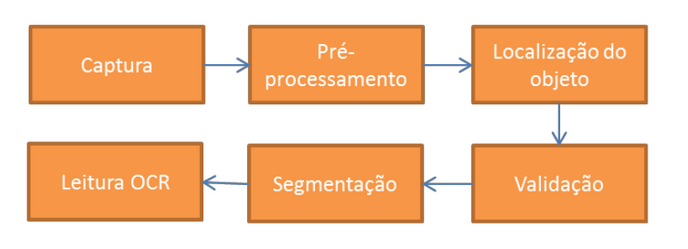
\includegraphics[width=.9\textwidth]{figuras/f1c1.png}
\end{center}
\legend{Fonte: \citeonline{licenseplaterecognition}}
\end{figure}


O autor fez uso da biblioteca Tesseract-OCR \cite{tesseract-ocr}, mostrando um desempenho consideravelmente bom, dependendo das circunstâncias em que se encontram as etapas de validação e segmentação. Porém, foram necessários treinamentos do Tesseract-OCR, que foram considerados ``trabalhosos'' pelo autor. Certos testes resultaram em falhas, devido a alguns problemas que serão citados ao longo do trabalho. 

Este trabalho então, tem como proposta principal implementar uma solução semelhante com o uso das bibliotecas de OCR "GOCR" e "OCRAD", testando dessa forma se é possível manter o desempenho em relação a biblioteca Tessaract-OCR sem a utilização de treinamentos. Vale enfatizar que o fato de utilizar diferentes OCRs afeta diretamente no resultado, podendo ser melhor ou não.

O restante desse trabalho está dividido em cinco capítulos. O capítulo 2 trata a respeito do que é visão computacional e OCR, explicando conceitos de forma geral e apresentando certas aplicações que o utilizam. O capítulo 3 explora a ferramenta OpenCV e suas funcionalidades dando ênfase nas que serão utilizadas para a solução, também serão vistas algumas questões sobre o GOCR o OCRAD e o Tesseract, e para conclusão do capítulo serão abordados conceitos básicos de processamento de imagens. O Capítulo 4 aborda o desenvolvimento. O capítulo 5 trata-se da conclusão.

\chapter{O que é visão computacional e OCR?}

Este capítulo apresenta os conceitos básicos de visão computacional e OCR. Não serão abordados a fundo como ambos funcionam, mas sim para que e onde são utilizados.  

\section{Visão computacional}

A Visão Computacional é um campo de estudo da computação que tem por objetivo tornar possível um computador ver e analisar imagens, extraindo informações úteis de componentes como uma câmera de vídeo, \textit{scanners} e dispositivos semelhantes \cite{computervision}. Em outras palavras, visão computacional tem o objetivo final de usar computadores para emular a visão humana, incluindo a aprendizagem e a capacidade de fazer inferências e tomar decisões baseadas nas entradas fornecidas. Essa área é um ramo que pertence à inteligência artificial, que por sua vez tem o objetivo central de emular a inteligência humana \cite{computervision}. A análise de uma imagem está entre o processamento de imagens e a visão computacional \cite{gonzalez}.

Entre processamento de imagens e visão computacional podem ser encontrados três níveis de processos, respectivamente, baixo-nível, nível-médio e alto-nível. Os processos de baixo-nível envolvem operações primárias, tais como a redução de ruído ou melhoria no contraste de uma imagem. Os processos de nível-médio são operações do tipo segmentação (particionamento da imagem em regiões) ou classificação (reconhecimento dos objetos na imagem). Os processos de alto-nível estão relacionados com as tarefas de cognição associadas com a visão humana \cite{gonzalez}.

Olhando para um grupo de pessoas em um porta-retratos, os seres humanos são capazes de identificar cada pessoa, reconhecer o nome e, através da expressão facial, até mesmo obter conhecimento do comportamento sentimental da pessoa naquele momento. Estudiosos passaram décadas tentando compreender como o sistema visual funciona, e chegaram a bons resultados em certas áreas como reconhecimento de texto. Mas ainda há muito para evoluir como na inteligência artificial de uma forma geral \cite{marr} \cite{palmer}.

Atualmente, com os avanços em visão computacional, pode-se identificar com alta probabilidade pessoas em meio a um cenário complexo, ou seja, que contenha diversos outros objetos incluídos, como árvores, carros, animais e outros, e dar-lhes os respectivos nomes. A \autoref{fig:recPessoas} ilustra a detecção de seis pessoas dentro de um barco, e a \autoref{fig:recCenario} ilustra um sistema capaz de reconhecer uma pessoa em meio a um cenário que contém árvores, prédio, cadeiras e outros objetos, circulando a cabeça, os braços, mãos e pernas. Entretanto, não é possível dizer ainda que visão computacional consegue emular a visão de uma criança de dois anos, devido principalmente, ao grande número de incógnitas para poucos dados \cite{caap}.

\begin{figure}[htb]
 \label{fig:reconhecimento}
 \centering
  \begin{minipage}{0.48\textwidth}
    \centering
    \caption{Reconhecimento de seis pessoas em um barco} \label{fig:recPessoas}
    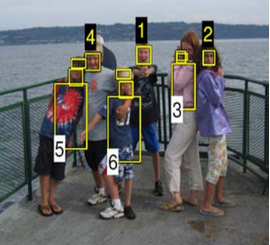
\includegraphics[width=.95\textwidth]{figuras/f1c2.png}
    \legend{Fonte:\citeonline{caap}}
  \end{minipage}
  \hfill
  \begin{minipage}{0.48\textwidth}
    \centering
    \caption{Reconhecendo e circulando pessoa em meio a cenário complexo} \label{fig:recCenario}
    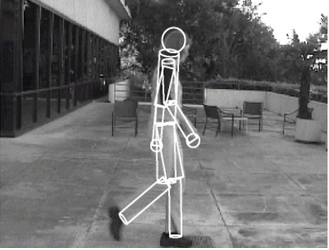
\includegraphics[width=.95\textwidth]{figuras/f2c2.png}
    \legend{Fonte: \citeonline{caap}}
  \end{minipage}
\end{figure}


%\begin{figure}[htbp]
%\caption{\label{fig:recPessoas} Reconhecimento de seis pessoas em um barco}
%\begin{center}
%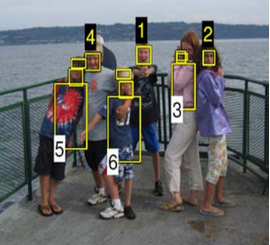
\includegraphics[width=.5\textwidth]{figuras/f1c2.png}
%\end{center}
%\legend{Fonte:\citeonline{caap}}
%\end{figure}

%\begin{figure}[htbp]
%\caption{\label{fig:recCenario}Reconhecendo e circulando pessoa em meio a cenário complexo}
%\begin{center}
%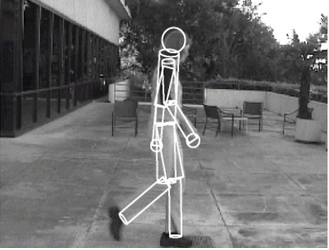
\includegraphics[width=.5\textwidth]{figuras/f2c2.png}
%\end{center}
%\legend{Fonte:\citeonline{caap}}
%\end{figure}

A visão computacional está sendo utilizada hoje em diversos meios, como \cite{caap}:


\begin{alineas}
\item no reconhecimento óptico de caracteres (OCR) aplicado a outros sistemas;
\item em sistemas de inspeção da máquina, em que são realizadas inspeções para garantia de qualidade, medindo as tolerâncias das asas de aviões, ou procurando defeitos em peças fundidas de aço, utilizando raios-X;
\item em construção de modelos 3D (fotogrametria) de forma totalmente automatizada a partir de fotografias aéreas utilizadas em sistemas como o Bing Maps \cite{bingmaps};
\item na radiologia é utilizado para registrar imagens pré-operatórias e intra-operatórias, ou na realização de estudos de longo prazo da morfologia do cérebro das pessoas à medida que envelhecem;
\item na área de segurança automotiva, tem-se o sistema de detecção de obstáculos inesperados, como pedestres na rua;
\item em jogos de movimentos, fundindo imagens geradas por computador com cenas de ação ao vivo por rastreamento de pontos característicos no vídeo fonte. Tais técnicas são amplamente utilizadas em Hollywood (por exemplo, filme Jurassic Park) \cite{robinandzafar};
\item em autenticação visual com o uso da \textit{webcan} para autenticação de usuário;
\item em câmeras digitais através da detecção facial, auxiliando a câmera digital a focar na região correta;
\item nos bancos, onde pode-se fazer autenticação por biometria, sendo as medidas biometricas a chave de segurança; 
\end{alineas}

\section{Reconhecimento ótico de caracteres}

Reconhecimento ótico de caracteres é uma das áreas que envolve visão computacional como analisado anteriormente. \citeonline{ocr} faz a seguinte definição de OCR:
\begin{citacao}	
O processo de reconhecimento óptico de caracteres (OCR) envolve o uso de sistemas de imagem e computadores para converter texto manuscrito ou impresso em texto que a máquina é capaz de codificar e reconhecer. OCR possui muitos usos, como a simplificação de entrada de dados, reconhecimento de placa de licença de veículos, e disponibilização de cópias editáveis de documentos impressos \cite{ocr}.
\end{citacao}
De maneira comercial, alguns sistemas OCRs começaram a surgir por volta de 1960, porém esses sistemas possuíam muitas limitações. Essa foi considerada a primeira geração de sistemas OCR. A segunda geração surgiu próxima do início de 1970, onde os sistemas OCRs já eram capazes de maneira singela, de reconhecer cartas escritas a mão. Pouco tempo depois, surge a terceira geração, dando resultados mais precisos sendo usados em \textit{scanners} \cite{eikvil1993optical}. Os estudos estão continuamente sendo feitos desde então buscando melhorias, mas não há registros muito relevantes, nem mesmo nomeações oficiais de novas gerações. 

Há dois tipos de sistemas que podem ser encontrados de forma geral com o uso de OCRs: sistemas de reconhecimento de caracteres offline (OffOCR) e sistemas de reconhecimento de caracteres online (OnOCR). Ambos são muito utilizados e sua diferença principal é bem clara. Os sistemas OffOCRs fazem o reconhecimento do texto depois de ser impresso ou escrito a mão, necessitando apenas iniciar um processo de escaneamento para então o reconhecimento propriamente dito. Já os sistemas OnOCRs fazem o reconhecimento ainda enquanto o texto está sendo produzido. Em relação aos sistemas OffOCRs, todos os detalhes das condições do texto que será escaneado são importantes pois afetam diretamente na qualidade do resultado \cite{shah2013literature}.

Todo o tipo de sistema OCR (OnOCR e OffOCR) passa pelos processos de entrada de dados, pré-processamento, segmentação, extração de traços, classificação e pós processamento, ilustrado na \autoref{fig:diagrama}.

\begin{figure}[htbp]
\caption{\label{fig:diagrama}Etapas efetuadas por um sistema OCR}
\begin{center}
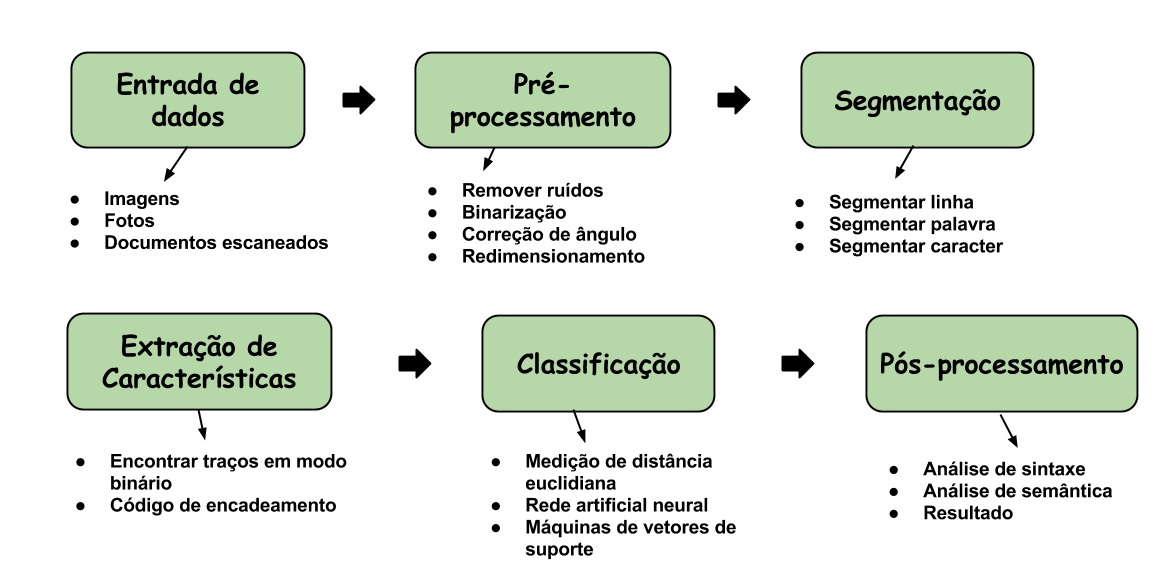
\includegraphics[width=.9\textwidth]{figuras/f3c2.png}
\end{center}
\legend{Fonte: o autor}
\end{figure}

As etapas ilustradas pela Figura 4 podem ser descritas da seguinte forma \cite{shah2013literature}:

\begin{alineas}
\item A etapa de entrada de dados é quando se adquire as imagens que serão analisadas, sejam fotografias, imagens coletadas de outras formas ou documentos escaneados. 
\item O pré-processamento é onde a imagem de entrada deve ser trabalhada para que esteja na melhor condição possível antes de chegar no ponto onde será segmentada. Isso envolve certos pontos importantes como a aplicação de \textit{filtros} utilizados em processamento de imagens como:
	\begin{subalineas}
		\item Remoção de ruídos: Erros de escaneamento, \textit{pixels} indesejados e problemas 			semelhantes são removidos ou tratados;
		\item Binarização (Limiarização): Processo que converte em preto e branco as imagens coloridas e que 	também ajuda no destacamento do caracter;
		\item Correção de ângulo: Adequa o ângulo para que os caracteres possam ser reconhecidos corretamente;
		\item Redimensionamento: Passo que auxilia principalmente em relação ao tempo de 					processamento.
	\end{subalineas} 
\item A segmentação é feita através de histogramas, dividida em duas partes, uma para identificar a linha onde estão as palavras e letras e outra para identificar colunas, separando caracter por caracter.
\item Extração de características é considerado o principal passo de extração de padrões em si. Dentro dessa fase encontram-se diversas técnicas, como a binarização, encadeamento dos resultados, histogramas dentre outros
\item A classificação recebe as informações da extração de características e com isto, mede a distância entre os pontos semelhantes e faz uma comparação com um padrão pré-armazenado que a própria OCR contém, buscando em que classe a informação recebida como entrada melhor se encaixa. A fórmula da distância entre os pontos \textit{euclidianos} será utilizada também em outras áreas no que diz respeito ao desenvolvimento deste projeto, e é dada por $ d(u , v) = |u - v| $ \cite{steinbruch1975algebra}.

\item O pós-processamento não é considerado como uma etapa essencial ou obrigatória. Porém pode ajudar num melhor resultado. Basicamente, trata de erros de caracteres muito parecidos, tais como a letra $O$ e o número $0$. 
\end{alineas}

As bibliotecas OCRs que serão usadas no desenvolvimento, providenciam a leitura OCR. Isso significa que elas são capazes de fazer as etapas de segmentação, extração de características e de classificação descritas no item b. As etapas de entrada de dados, pré-processamento e pós-processamento são necessárias para aumento da taxa de acerto, e serão realizadas através da biblioteca OpenCV em conjunto com o Python.

A \autoref{fig:filtros} representa os principais filtros usados na etapa de pré-processamento. O item (a) indica uma imagem original, o item (b) a imagem passada pelo processo de dilatação, o item(c) pelo processo de erosão, o item (d) pelo processo de maioria, o item (e) pelo processo de abertura e por fim o item (f) passa pelo processo de fechamento. Alguns destes processos serão utilizados posteriormente na sessão de desenvolvimento, consequentemente receberão um melhor detalhamento de como funcionam na prática \cite{caap}.

\begin{figure}[htbp]
\caption{\label{fig:filtros}Filtros de processamento de imagens aplicados a uma imagem}
\begin{center}
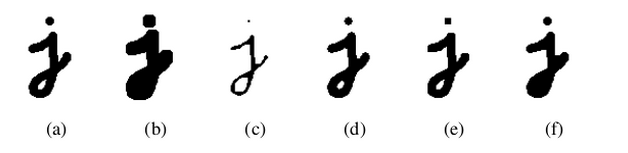
\includegraphics[width=.9\textwidth]{figuras/f4c2.png}
\end{center}
\legend{Fonte: \citeonline{caap}}
\end{figure}

\section{Conclusão}

Nesse capítulo foram apresentados conceitos fundamentais sobre visão computacional dando exemplos de onde se é aplicado. Também foram analisados os conceitos básicos de um sistema OCR. O próximo capítulo tem o objetivo de demonstrar certas ferramentas que serão aplicadas no capítulo de desenvolvimento.

\chapter{Ferramentas}

Este capítulo introduz as ferramentas que serão utilizadas ao longo do desenvolvimento. Descreve-se aqui o OpenCV e suas funcionalidades principais, dando ênfase em funções que fazem parte da solução. Também são demonstradas as bibliotecas de OCR GOCR \cite{GOCR}, OCRAD \cite{OCRAD} e Tesseract \cite{tesseract-ocr}.

\section{O OpenCV}

O OpenCV é uma biblioteca de visão computacional disponível de forma gratuita, escrita na linguagem de programação C e \cpp, sendo ela multiplataforma podendo ser usada em qualquer distribuição Linux, Windows e Mac OS X. O OpenCV pode ser integrado em linguagens como o Python, Ruby, Matlab, C e \cpp, dentre outras \cite{learningopencv}. Ele teve início como um projeto de pesquisa da Intel \cite{intel} no ano de 1998, ficando disponível com licença BSD em 2000. Foi registrado que o download dessa biblioteca foi efetuado mais de três milhões de vezes até 2012 \cite{pulli2012real}, e até hoje vem crescendo e tem sido usado por profissionais da área, professores e estudantes.

Projetado para ter um bom desempenho diante de aplicações em tempo real, o OpenCV trabalha bem com processadores Intel. A própria empresa vende determinadas bibliotecas extras para melhorias em relação ao desempenho do OpenCV. Um dos principais objetivos do OpenCV é providenciar uma infraestrutura de visão computacional que auxilia profissionais específicos da área, professores e estudantes a desenvolverem sistemas sofisticados com simplicidade e eficiência, disponibilizando mais de quinhentas funções como por exemplo, inspeção de produtos de fábrica, imagem médica, segurança, interface para usuários, calibração de câmera, visão estéreo e robótica \cite{learningopencv}. 

\subsection{Funcionalidades do OpenCV}

Algumas das funcionalidades do OpenCV serão exibidas nesta sub-sessão, todos os códigos deste e de outros capítulos estão na linguagem Python 2.7.2. Como analisado, existem mais de quinhentas funções no OpenCV, contudo, serão analisadas apenas algumas funções gerais de processamento de imagens e um exemplo de aplicação.

\subsection{Dilatação e Erosão}	
O OpenCV disponibiliza funções de filtros que serão abordados na sessão de desenvolvimento, um destes é conhecido como dilatação (\autoref{fig:dilatacao}). De acordo com os autores \cite{oge1999processamento} para compreender a fórmula matemática de dilatação faz-se necessário compreender também os seguintes conceitos:

\begin{figure}[htbp]
\caption{\label{fig:dilatacao}Demonstração do efeito de dilatação sobre um \textit{pixel}}
\begin{center}
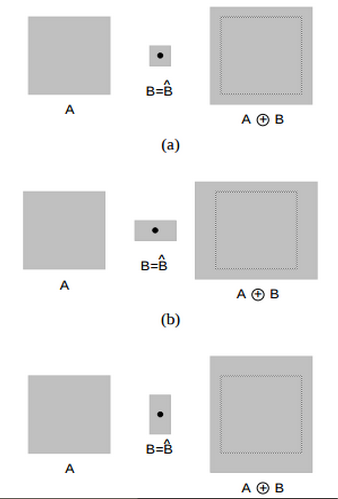
\includegraphics[width=.3\textwidth]{figuras/f1c3.png}
\end{center}
\legend{Fonte: \citeonline{oge1999processamento}}
\end{figure} 

Sejam $A$ e $B$ conjuntos no espaço $ Z^2 $ onde respectivamente $A = (a1 , a2)$ e $B = (b1 , b2)$, e seja $\emptyset$ o conjunto vazio. A denotação $(A)_x$ é definida pela translação de $A$ por um $x$ qualquer onde $x = (x1 ,  x2)$. Tem-se:
\[
(A)_x = \{c | c = a + x\}, \mbox{para~} a \in A
\]
Isso quer dizer que, se $x$ supostamente fosse igual ao ponto $(1,2)$ e $A$ fosse igual ao ponto $(3,3)$ a translação de $A$ por $x$ seria igual ao ponto $(4,5)$. Todos os \textit{pixels} se deslocariam de $A$ até $x$, resultando no ponto encontrado ao fim da equação.

A reflexão de $B$ é dada por:
\[
\hat{B} = \{x | x = -b \mbox{ para } b \in B\}
\]
Logo, a reflexão de $B$ trata-se da rotação de 180\textordmasculine \hspace{} em relação a origem.

O Complemento de $A$ é:
\[
A^c = \{x | x \not \in A\}
\]

Ou seja, o complemento de $A$ são os pixels que não pertencem a $A$, em uma imagem binária (preto e branco) corresponderia aos \textit{pixels} brancos da figura caso o objeto principal fosse em preto como na \autoref{fig:filtros2}(b).

\begin{figure}[htbp]
\caption{\label{fig:filtros2}Filtros de dilatação e erosão sobre uma imagem}
\begin{center}
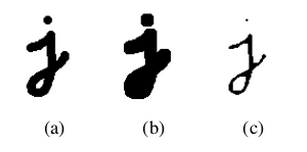
\includegraphics[width=.5\textwidth]{figuras/f3c3.png}
\end{center}
\legend{Fonte: \citeonline{caap}}
\end{figure} 

A diferença entre $A$ e $B$ é definida por:
\[
A - B = \{x | x \in A,x \not \in B\} = A \cap B^c
\]
Portanto, sendo a diferença de $A$ e $B$ igual a intersecção de $A$ por complemento de $B$, essa diferença será os pontos em comum de $A$ e complemento de $B$. Com os conceitos apresentados compreendidos, segue a fórmula da dilatação:

\[A \oplus B = \{x|(\hat{B})_x \cap A \notin \emptyset\}\]

\noindent onde que $A$ representa a imagem a ser operada, e $B$ é um segundo conjunto de pixels, de uma forma que opera sobre os pixels de A para produzir o resultado. O conjunto B é chamado de elemento estruturante. A dilatação de $A$ por $B$ é o conjunto de todos os deslocamentos de $x$ tais que $A$ sobreponham-se em pelo menos um elemento não nulo.


No OpenCV, a dilatação pode ser aplicada de maneira simples, dando apenas duas entradas de dados, sendo elas a própria imagem e o kernel. O Kernel\footnote{Matriz de convolução utilizada para borrar, controlar nitidez dentre outras funções. No caso desse trabalho, define a expessura da dilatação e da erosão \cite{shapiro2001computer}.} de maneira bem resumida definirá a espessura do resultado final, basicamente é responsável por definir o quanto será dilatada a imagem \cite{opencv}. O Código 1 é um código de dilatação de uma imagem, onde inicia-se importando as bibliotecas OpenCV e Numpy, respectivamente cv2 e np. Após a importação das bibliotecas principais, uma variável chamada ``img'' utiliza a função \textit{imread} do OpenCV, que apenas faz uma leitura da imagem ``j.png'' em escala de cinza, definida pelo parâmetro ``0''. Assim define-se o \textit{kernel} e por fim a dilatação, feita através da função \textit{dilate} também do OpenCV. Segue o código comentado:

\lstinputlisting[language=python,caption={Dilatação de uma imagem},label=mediapy]{codigos/dilate.py}

A erosão é o inverso da dilatação. Se por um lado o efeito da dilatação adiciona pixels a um objeto, a erosão retira \cite{parker10@algorithms}. O efeito da erosão pode ser observado na \autoref{fig:filtros2}(c). A fórmula matemática do efeito de erosão é:

\[ A \ominus B = \{c|(B)_c \subseteq A\} \]

O conjunto $A \ominus B$ é o conjunto de translações de B que se alinham sobre um conjunto de pixels pretos em $A$. Isto significa que nem todas as translações devem ser consideradas, mas apenas aquelas que, sobrepõe a origem de $B$ em um dos membros de $A$. \cite{parker10@algorithms}. Abaixo segue o Código 2, sendo ele muito semelhante ao Código 1, apenas diferenciando-se na aplicação final da função do OpenCV \textit{erode} no lugar da função \textit{dilate}.

\lstinputlisting[language=python,caption={Erosão de uma imagem com base na fonte},label=mediapy]{codigos/erosion.py}

Observa-se que as funções de dilatação e erosão são aplicadas de forma praticamente idêntica. Não existe apenas uma forma de aplicar dilatação e erosão, pelo contrário, outras fórmulas dependente da situação podem ser encontradas \cite{parker10@algorithms}, entretanto de forma geral estas apresentadas são base para compreensão do tema.


\subsection{Limiarização - Thresholding}

Limiarização\footnote{Alguns autores traduzem o termo como \textit{binarização}} é um método de segmentação baseado em similaridade de níveis de cinza, buscando extrair objetos de interesse mediante a definição de um limiar $T$ que separa os agrupamentos de níveis de cinza da imagem. A segmentação se dá varrendo a imagem, pixel a pixel, e rotulando cada pixel como sendo do objeto ou do fundo, em função da relação entre o valor do pixel e o valor do limiar \cite{IntroProcessDigIMG}. Limiarização é computacionalmente barato e rápido, é o método de segmentação mais antigo e ainda é amplamente utilizado em aplicações simples. Pode facilmente ser usado em tempo real. Limiarização é a transformação da imagem $f$ para obter como saída a imagem $g$, como pode ser visto na fórmula abaixo \cite{sonka2014image}:

\[
g(i,j) = 1 \mbox{~para~} f(i,j) > T 
\]
\[
g(i,j) = 0 \mbox{~para~} f(i,j) \leq T
\]

Em que $T$ é o limiar que é definido conforme o histograma da imagem e também de acordo com quantos objetos se quer extrair da imagem, e os pontos $g$ e $f$ representam pixels da imagem $g$ e da imagem $f$. Quando $g(i,j)$ é igual a $0$, caracteriza o fundo da imagem, e quando $g(i,j)$ é igual a $1$, caracteriza-se o objeto \cite{sonka2014image}.

Este método de limiarização apresentado, é mais simples. Há outros métodos de limiarização, basicamente a diferença entre eles é a forma ou solução para encontrar o limiar $T$. O OpenCV disponibiliza cinco tipos diferentes de limiarização que são demonstrados no Código 3 e na \autoref{fig:limiar} \cite{opencv}. Não serão explicados aqui detalhes a respeito de todas as limiarizações, apenas uma pequena demonstração de cada uma. 

Para que os códigos apresentados no Código 3 façam sentido, faz-se necessário o conhecimento básico do que é a biblioteca Matplotlib. Matplotlib é uma biblioteca de geração de gráficos bidimensional Python, que produz figuras de qualidade de publicação, em uma variedade de formatos e em várias plataformas. O Matplotlib permite gerar gráficos, histogramas, espectros de potência, gráficos de barras, gráficos de dispersão e outras funções \cite{Hunter:2007}. 

O Código 3 possui além das importações já comentadas anteriormente, a importação do matplotlib na linha 6. A leitura de uma imagem chamada ``31.jpg'' é feita, e então da linha 9 até a linha 13 são aplicadas as funções de limiarização disponíveis no OpenCV. Os valores 127 e 255 são \textit{limiares} utilizados de forma geral por padrão para aplicar limiarização em imagens. O matplot é utilizado apenas para apresentar essas imagens uma ao lado da outra como pode ser verificado na \autoref{fig:limiar}. Na linha 15 do Código 3, uma lista de nomes são agregados a uma lista de cada imagem \textit{limiarizada}, e ambos são apresentados através do MatPlot nos comandos da linha 18 até a 22. Segue o Código 3:

\lstinputlisting[language=python,caption={Thresholding em uma placa},label=mediapy]{codigos/thresholding.py}

\begin{figure}[htbp]
\caption{\label{fig:limiar}Thresholding(Limiarização) sobre uma imagem de uma placa}
\begin{center}
	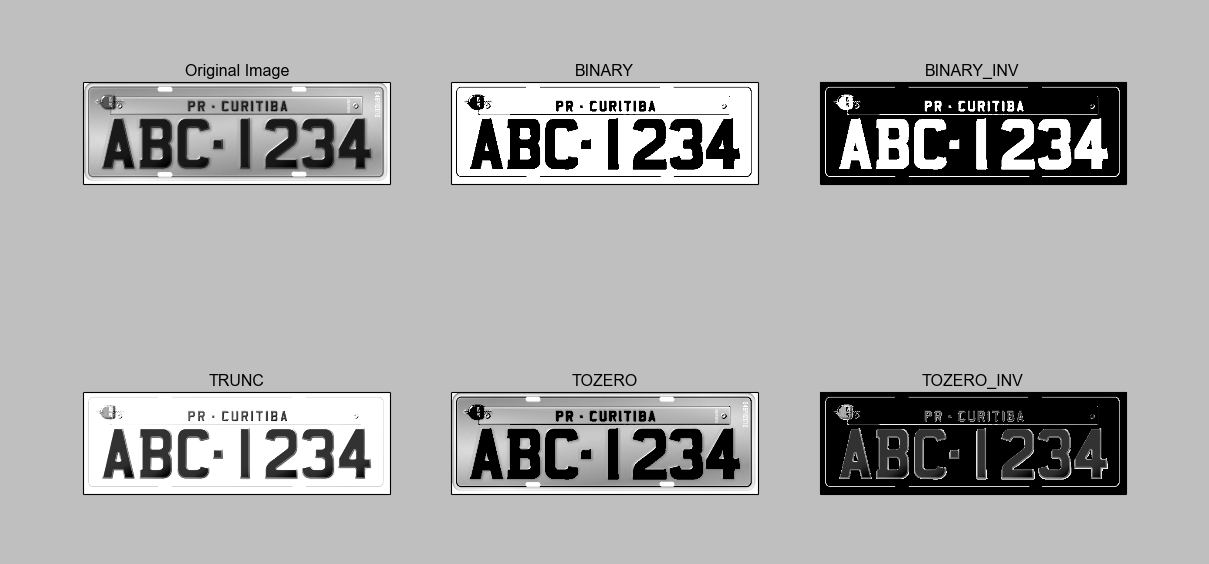
\includegraphics[width=.9\textwidth]{figuras/f2c3.png}
\end{center}
\legend{Fonte: o autor}
\end{figure} 
 
\subsection{Detecção de bordas, Histogramas e Detecção de cores}

Detecção de bordas Canny é um dos algoritmos de detecção de borda que o OpenCV dispõe, e será usado aqui como exemplo embora existam outros algoritmos que possam ser tão úteis quanto ele. Ele foi desenvolvido por John F. Canny em 1986. É um algoritmo que passa por alguns estágios antes de sua solução final. Iniciando pela remoção de ruídos, encontrando a intensidade do gradiente da imagem, removendo pixels indesejados e finalmente encontrando as bordas \cite{opencv}. 

Para utilizar o algoritmo de Canny, basta fazer uso da função ``cv2.Canny'' como feito na linha 6 do Código 4. Os valores 100 e 200 observados na linha 6, são também valores utilizados por padrão. A \autoref{fig:deteccao_bordas} representa o resultado do Código 4 sobre uma imagem.

\lstinputlisting[language=python,caption={Detecção de bordas Canny, resultado representado pela Figura 9},label=mediapy]{codigos/deteccaobordas.py}

\begin{figure}[htbp]
\caption{\label{fig:deteccao_bordas}Resultado do código de Detecção de bordas sobre uma imagem de uma placa}
\begin{center}
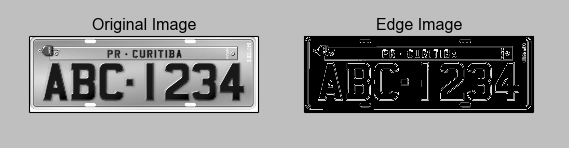
\includegraphics[width=.9\textwidth]{figuras/f4c3.png}
\end{center}
\legend{Fonte: o autor}
\end{figure} 

Além dessa função de detecção de bordas o OpenCV disponibiliza visualização de histogramas, que são lidos através da biblioteca MatPlotLib. O histograma é uma das mais comuns formas de representação das distribuições de pixel em uma imagem. Quando observado é possível obter instantâneamente noções das características da imagem em questão, podendo inferir informações relevantes, como a intensidade das cores \cite{neta2008limiarizaccao}.

O Código 5 é um exemplo de código utilizando a mesma placa da \autoref{fig:deteccao_bordas} e sequencialmente a \autoref{fig:resultado_histograma} apresenta o resultado do código. É possível verificar na linha 6 que para apresentar o histograma basta utilizar a função \textit{hist} da MatPlotLib:


\lstinputlisting[language=python,caption={Histograma, resultado representado pela Figura 10},label=mediapy]{codigos/histogramas.py}

\begin{figure}[htbp]
\caption{\label{fig:resultado_histograma}Resultado do código de histrograma}
\begin{center}
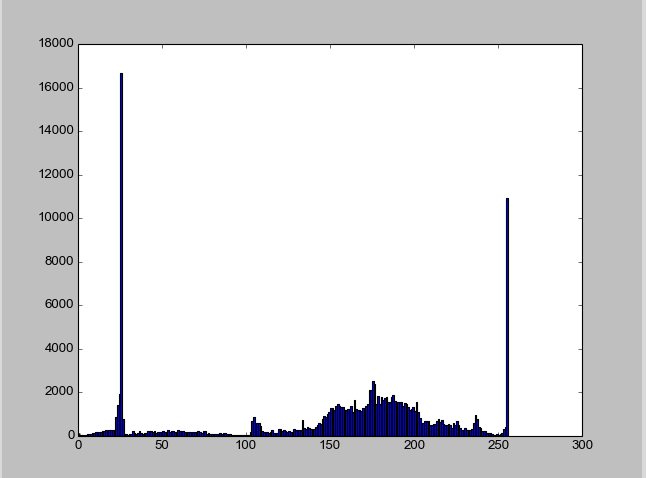
\includegraphics[width=.9\textwidth]{figuras/f5c3.png}
\end{center}
\legend{Fonte: o autor}
\end{figure} 

Para concluir a sessão do OpenCV, será mostrado uma pequena aplicação que destaca apenas a cor azul de objetos que possam estar em frente a câmera. Pode-se notar que neste caso não é aberta uma imagem como entrada, mas sim captura direta da câmera, ou seja, tempo real. Este código não trabalha com o padrão RGB(\textit{red green blue}) de cores, mas sim o padrão conhecido como HSV(\textit{hue saturation value}). 

Na linha 4 do Código 6 é iniciada a leitura da câmera, e então na linha 6 é criado um laço sem finalização. A linha 9 captura cada \textit{frame} da câmera, e em na linha 12 é convertido para o padrão HSV. As linhas 15 e 16 definem os valores da cor azul, e na linha 19 é aplicada a função inRange para extrair apenas essa cor. A partir da linha 22 são apenas utilizados códigos para a apresentação na tela. O representação do resultado está na \autoref{fig:deteccao_cor}.

\lstinputlisting[language=python,caption={Encontrando objetos da cor azul, resultado representado pela Figura 11},label=mediapy]{codigos/findblue.py}

\begin{figure}[htbp]
\caption{\label{fig:deteccao_cor}Resultado do código de detecção de cor azul}
\begin{center}
	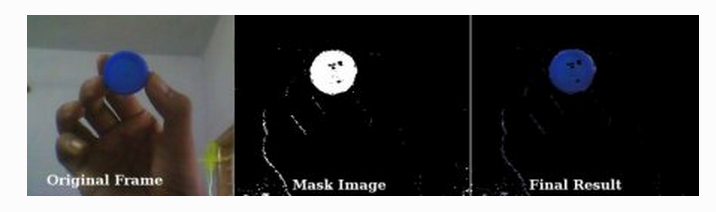
\includegraphics[width=.9\textwidth]{figuras/f6c3.png}
\end{center}
\legend{Fonte: \citeonline{opencv}}
\end{figure} 

\section{O GOCR e o OCRAD}

Nos dois capítulos anteriores, já foram identificadas as funções de uma OCR, e também foram citados os nomes de algumas bibliotecas OCR. O GOCR e o OCRAD sendo algumas dessas bibliotecas compõe parte importante neste trabalho, haja visto que trata-se da comparação de uma solução que não possui treinamento de reconhecimento de novos caracteres, utilizando ambas as bibliotecas, e uma solução utilizando o Tesseract(especificado na próxima sessão) com o uso de treinamento. 

O GOCR é um motor OCR desenvolvido sob a Licença Pública GNU. Ele converte imagens digitalizadas de texto em arquivos de texto manipuláveis. Joerg Schulenburg foi quem criou a ferramenta, e passou a liderar uma equipe de desenvolvedores que procuraram melhorar a qualidade do GOCR. O GOCR pode ser usado em diferentes sistemas operacionais e arquiteturas. Ele pode abrir muitos formatos de imagem diferentes. Sua atualização mais recente é de 05/03/2013, sendo nomeada de "GOCR 0.50", estando disponível para download no site oficial \cite{GOCR}.

O OCRAD também é um motor OCR de licença GNU, com base em um método de extração de características. A leitura de imagens são pelas extensões PBM(bitmap), pgm(escala de cinza) ou ppm(colorida) e extrai o texto nos formatos byte ou UTF-8. Também inclui um analisador de layout capaz de separar as colunas ou blocos de texto normalmente encontrados nas páginas impressas. Ocrad pode ser usado como um aplicativo de console autônomo, ou como um \textit{backend} para outros programas. Assim como o GOCR, também pode-se contribuir para o melhoramento desse programa\cite{OCRAD}. O OCRAD também tem um manual online em sua página oficial.

\section{Tesseract}

Tesseract é o motor OCR de licença gratuita desenvolvido pela HP(Hewlett-Packard) \cite{Hewlett-Packard} por volta de 1984 e 1994. Foi modificado e melhorado em 1995 tendo bons resultados. Tornou-se verdadeiramente licença gratuita em 2005. Hoje pertencente oficialmente a Google, o Tesseract possui suporte a diversas linguagens, tendo que ser treinado para o caso específico no qual esteja sendo submetido, para assim gerar os resultados desejados\cite{patel2012optical}.

\subsection{Conclusão}

Nesse Capítulo foram apresentadas as ferramentas que serão utilizadas no Capítulo 4. Alguns exemplos práticos foram citados e demonstrados. Cada exemplo possui um código e uma imagem que demonstra o respectivo resultado.
\chapter{Desenvolvimento}

Neste capítulo serão abordadas as principais instalações e metodologias para a implementação dessa solução.

\section{Principais instalações}

Como descrito anteriormente, o sistema operacional utilizado para essa solução é o GNU/Linux Ubuntu 14.04. São necessárias as bibliotecas OpenCV 3.0 GOCR 0.50 e OCRAD 0.22. 

\subsection{OpenCV 3.0}

Para instalar o OpenCV 3.0 são necessárias algumas dependências, para isso basta utilizar o Código 7 no terminal:

\lstinputlisting[language=terminal,caption={Comandos terminal - Dependências OpenCV},label=mediapy]{codigos/installopencv}

Após instaladas todas as dependências, deve-se criar um diretório onde será instalado o OpenCV como observado na linha 1 do Código 8. Dentro desse diretório, via terminal, o próximo passo é fazer o \textit{download} \cite{opencv} do OpenCV visto na linha 3.

\lstinputlisting[language=terminal,caption={Comandos terminal - Download OpenCV},label=mediapy]{codigos/installopencv2}

Quando o \textit{download} for concluído, os comandos do Código 9 devem ser executados no terminal. Esse processo está apenas criando novo diretório onde definitivamente instala o OpenCV através do comando \textit{Make}.

\lstinputlisting[language=terminal,caption={Comandos terminal - Processo de instalação I},label=mediapy]{codigos/installopencv3}

Para concluir a instalação, precisa-se ainda dos comandos do Código 10. Esses comandos têm a função de construir um \textit{cache} das bibliotecas no sistema. 

\lstinputlisting[language=terminal,caption={Comandos terminal - Processo de instalação II},label=mediapy]{codigos/installopencv4}

Dessa forma, o OpenCV 3.0 já estará pronto para uso, ao reiniciar o sistema operacional é possível testá-lo ao acessar a pasta \textit{examples} dentro do diretório onde foi feita a instalação.

\subsection{GOCR e OCRAD}

As bibliotecas GOCR e OCRAD já estão nos repositórios do Ubuntu 14.04, e as versões que estão sendo utilizadas nessa solução são as mais recentes. Nesse caso, os únicos comandos necessários para instalação completa dessas ferramentas são apresentados no Código 11.

\lstinputlisting[language=terminal,caption={Comandos terminal - Instalando o GOCR e o OCRAD},label=mediapy]{codigos/installGocrOcrad}

Considerando que o Python já vem instalado na distribuição e pronto para uso, não são mais necessárias outras instalações para a implementação da solução.

\section{Metodologia}

Essa sessão tratará da metodologia para a solução proposta, contendo os códigos e a forma como foram obtidas as imagens. 

\subsection{Solução}

Para uma melhor compreensão, a solução pode ser dividida nas seguintes etapas:

\begin{alineas}
\item obtenção da imagem;
\item tratamento da imagem;
\item leitura OCR;
\item tratamento da saída das OCRs.
\end{alineas}

A obtenção da imagem é a etapa mais simples de se compreender. Qualquer dispositivo com a função de fotografar pode ser usado como meio de fornecer as imagens, desde câmeras de dispositivos móveis, até \textit{webcams} USB e câmeras digitais propriamente ditas, em qualquer nível de resolução. No caso dos testes realizados para esse trabalho, foram utilizadas câmeras de dispositivos móveis com a resolução de três megapixels. Essa imagem será a entrada da solução, e o próximo passo, que será o tratamento da imagem, necessariamente utilizará as funções do OpenCV. Dessa forma, a imagem de entrada deverá ser lida diretamente pelo OpenCV.

Para que o Python e o OpenCV estejam conectados é preciso que no código Python estejam importadas as bibliotecas que serão utilizadas. É importado então o OpenCV, chamado de \textit{cv2}, o Numpy, chamado de \textit{np}, e o Matplotlib como \textit{plt}. Dessa forma poderá ser usado qualquer função do OpenCV do Numpy e do Matplotlib no restante do código. Após essas importações, uma imagem já pode ser lida através do OpenCV pela função \textit{imread}. Ao verificar essas importações no Código 12, percebe-se que na função imread na linha 8 há dois parâmetros, um sendo o caminho relativo da imagem e o outro o valor 0, esse valor 0 representa que a imagem será lida em escala de cinza. O fato de estar em escala de cinza, facilita o processo de limiarização analisado no capítulo anterior, devido a imagem ter menos variações de cores.

\lstinputlisting[language=Python,caption={Código da Solução I - Importações e leitura},label=mediapy]{codigos/implementacao.py}

É válido citar que não serão descritas todas as linhas de código, mas sim as funções e alguns detalhes importantes, porém o código completo estará disponível em anexo. A solução inicia chamando a função \textit{"tratamento"}(Código 13), que trata-se da etapa de tratamento da imagem. É importante dizer que nesse caso em específico, estão apenas sendo utilizadas imagens anteriormente fotografadas, mas pode-se fazer essa etapa em tempo real, pois o OpenCV disponibiliza a função \textit{VideoCapture} que faz uso de qualquer dispositivo de câmera disponível, e também a função \textit{imwrite} que é capaz de salvar o que está sendo capturado através da câmera.

\lstinputlisting[language=Python,caption={Código da Solução II - Função principal},label=mediapy]{codigos/implementacao1.py} 

A etapa de tratamento da imagem efetua os filtros de remoção de ruídos, limiarização, dilatação, e erosão, exatamente nessa ordem, citados anteriormente nos capítulos 2 e 3. O filtro de remoção de ruídos pode ser encontrado em \cite{pcvwp} na página 23. Cada filtro é salvo através da função \textit{imread} do OpenCV. É importante destacar que a remoção de ruídos é aplicada sobre a imagem original e é salva como \textit{remocao.png}, então \textit{remocao.png} é lido e aplicado o filtro de limiarização, e assim sucessivamente. A Figura 12 ilustra os arquivos que são lidos, o filtro que é aplicado, e o nome salvo após a aplicação do novo filtro, deixando mais claro. O Código 14 é uma demonstração da função de tratamento da imagem.

 
\begin{figure}[htbp]
\centering
\caption{Sequência de aplicação de filtros}
\vspace{0.5cm}
\begin{tabular}{|r|c|c|c|}
\hline   
Ordem & Leitura & Filtro Aplicado & Escrita &
\hline                              
1º  &  Arquivo original & Remoção de ruídos & remocao.png & 
\hline
2º & remocao.png & Limiarização & limiar.png   &
\hline
3º & limiar.png  & Dilatação & dilatado.png  &
\hline
4º & dilatado.png & Erosão & erodido.png &
\hline
\end{tabular}
\legend{Fonte: o autor}
\end{figure}

\lstinputlisting[language=Python,caption={Código da Solução III - Função de Tratamento},label=mediapy]{codigos/implementacao2.py}

Depois de aplicados os filtros, as imagens salvas ficam como as que estão representadas na \autoref{fig:Imagens após o tratamento}. Essas imagens tratadas geram resultados muito melhores ao passar pelas OCRs, sendo que quando a imagem original não tratada é passada pelas OCRs, praticamente não são encontrados os caracteres. 

Assim é possível iniciar a próxima etapa, que é a de leitura OCR. Cada imagem salva passará pela leitura OCR, pois existe a possibilidade de que as letras e os números de interesse sejam encontrados em um filtro, e não em outro. 

\begin{figure}[htbp]
\caption{\label{fig:Imagens após o tratamento}Imagens após o tratamento da placa via OpenCV e Python}
\begin{center}
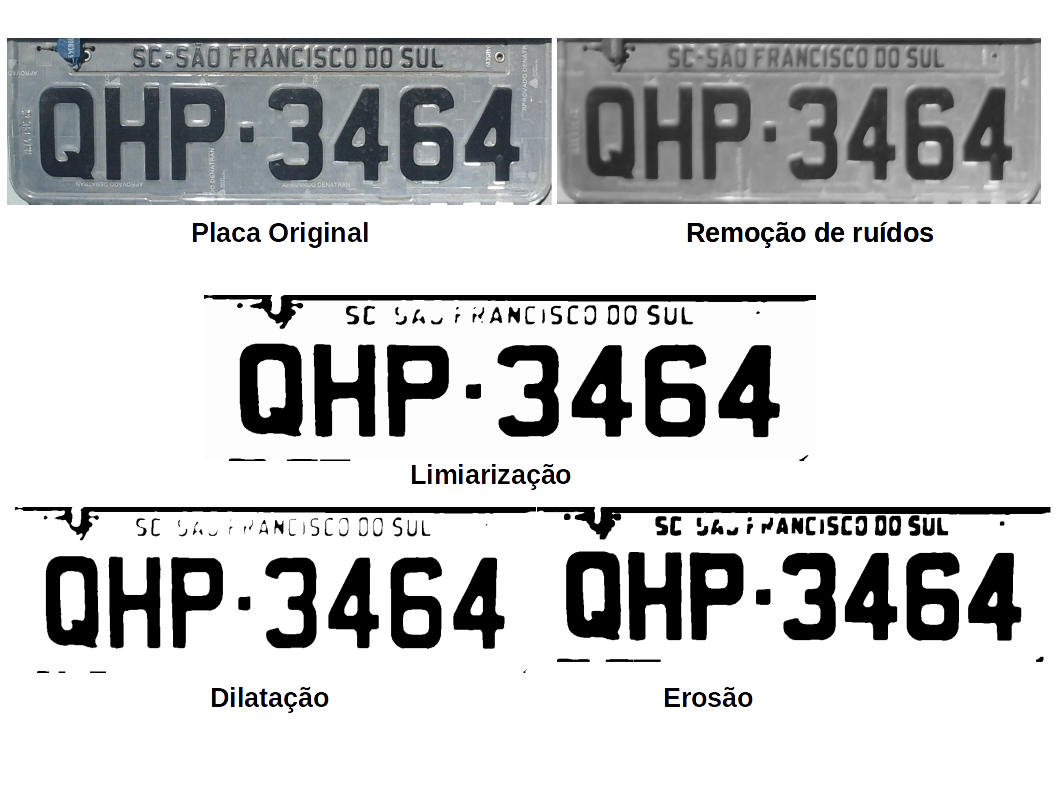
\includegraphics[width=.7\textwidth]{figuras/f1c4.png}
\end{center}
\legend{Fonte: o autor}
\end{figure}

A execução da leitura OCR através do Python é simples de fazer; basta importar a biblioteca \textit{commands} e executar o comando de leitura OCR que pode ser executado também no terminal do Linux. A biblioteca \textit{commands} permite a execução de quaisquer comandos do sistema operacional. O Código 15 é uma função de busca das saídas da leitura OCR.

\lstinputlisting[language=Python,caption={Código da Solução IV - Função de leitura OCR},label=mediapy]{codigos/implementacao3.py}

O último passo a ser dado para a implementação, é o tratamento das saídas da leitura OCR. As vezes a leitura OCR encontra pixels indesejados e os traz como resultado, o que atrapalha muito para encontrar os valores que realmente interessam. A Figura 14 representa um exemplo de um dos piores casos testados, e é de grande importancia para compreensão. É possível notar que letras que representam o nome do estado e da cidade são reconhecidos e retornados, também é perceptível que letras podem ser confundidas com números.


\begin{figure}[htbp]
\centering
\caption{Formato de respostas da leitura OCR}
\vspace{0.5cm}
\begin{tabular}{|r|c|}
\hline   
Informação da placa & SC - SÃO FRANCISCO DO SUL - MJC - 1865 & 
\hline                              
Dilatação OCRAD  &  r MJ\_C. l?Qs &
\hline
Erosão OCRAD & \_\_\_\_    \_\_\_J\_C\_ l \_\_6 5 & 
\hline
Limiarização OCRAD & MJ\_C.l?QS &
\hline
Dilatação GOCR & \_\_ \_    \_  \_ \_J\_C\_ l 8\_6 5 &
\hline
Erosão GOCR & \_\_\_\_      \_\_J\_C\_ l \_\_0 5 &
\hline
Limiarização GOCR & \_\_\_  \_\_  l \_J\_C l 8\_6 5 & 
\hline
\end{tabular}
\legend{Fonte: o autor}
\end{figure}

Na Figura 14, observa-se que na imagem que contém o filtro de dilatação, a leitura feita pelo OCRAD trouxe um pequeno ``r'' na frente do ``MJ\_C'' que são os caracteres de interesse, isso é um fator que complica muito a decisão de quais são os caracteres que realmente correspondem as letras de registro da placa, e não as de informação de estado e cidade. É possível verificar que os únicos filtros que conseguiram as letras, foram a dilatação através do OCRAD e a limiarização também pelo OCRAD, em contrapartida, os únicos filtros que conseguiram os números completos, foram os de dilatação via GOCR e limiarização também através do GOCR. Um detalhe que será explorado na conclusão, é que as letras ``MJC'' e os números ``1865'' apareceram duas vezes, e nos testes realizados, em todas as vezes que foi feita uma leitura OCR pelo menos uma vez as letras e os números apareceram em um dos filtros.

Para resolver essa situação encontrada, são necessárias duas funções, uma para encontrar as letras e outra para encontrar os números. Isso se deve a alguns erros comuns que ocorrem nas OCRs, como confundir a letra ``O'' com o número ``0''. A Figura 15 demonstra alguns dos erros mais comuns encontrados nos testes.

\begin{figure}[htbp]
\centering
\caption{Erros frequentes de leitura OCR}
\vspace{0.5cm}
\begin{tabular}{|r|c|}
\hline   
Letras & Números & 
\hline                              
O  &  0 &
\hline
l,I,i & 1 & 
\hline
B & 8 &
\hline
b, & 6 &
\hline
S,s & 5 & 
\hline
T & 7 & 
\hline
\end{tabular}
\legend{Fonte: o autor}
\end{figure}

Assumindo que esses erros apresentados são comuns, e que de maneira geral se conhece alguns erros como pontos, vírgulas, traços, interrogações e outros, a primeira ação no caso das letras é encontrar os caracteres incorretos e eliminá-los juntamente com os números, apenas deixando as letras maiúsculas. Essa limpeza resultaria nas saídas representadas na Figura 16.

\begin{figure}[htbp]
\centering
\caption{Primeira etapa de limpeza}
\vspace{0.5cm}
\begin{tabular}{|r|c|}
\hline   
Informação da placa & SC - SÃO FRANCISCO DO SUL - MJC - 1865 & 
\hline                              
Dilatação OCRAD  & MJCQ &
\hline
Erosão OCRAD & JC & 
\hline
Limiarização OCRAD & MJCQS &
\hline
Dilatação GOCR & JC &
\hline
Erosão GOCR & JC &
\hline
Limiarização GOCR & JC & 
\hline
\end{tabular}
\legend{Fonte: o autor}
\end{figure}

Nesse caso, onde houver no mínimo três caracteres, o resultado será os três primeiros, porém nem sempre os três primeiros serão as letras da placa, podendo ser uma letra da cidade ou estado como descrito anteriormente. Para os números o processo é semelhante, há uma limpeza de todas as letras e outros caracteres, deixando apenas os números e as letras que são geralmente confundidas(Figura 15) já substituídas pelo possível valor correto. No caso dos números, há uma taxa de acerto maior em relação as letras. O Código 14 demonstra um exemplo de função de limpeza para letras. Nesse código é utilizado somente a linguagem de programação, sem bibliotecas específicas para auxílio da tarefa.

\lstinputlisting[language=Python,caption={Código da Solução V - Exemplo de limpeza de letras},label=mediapy]{codigos/implementacao3-1.py}

Dessa forma, o último passo é juntar os resultados e retornar a resposta, após isso, a solução está encerrada no estágio atual. A próxima sessão tem por objetivo apresentar os resultados obtidos.

\section{Resultados}

Essa sessão apresentará os resultados parciais, considerando que a solução pode ser continuada e melhorada. 

A Tabela 1 mostra a taxa de acerto de três maneiras, sendo elas a placa completa, somente as letras e somente os números. Foram testadas trinta e cinco placas, em condições climáticas diferentes e em movimentação, fazendo uso de dispositivos móveis com no máximo oito \textit{megapixels}. A taxa de acerto pode ser considerada baixa, devido ao problema citado na sessão anterior a respeito das letras que pertencem ao estado e a cidade contidos na placa. 

Não existe um padrão de respostas, as letras podem estar em qualquer posição, misturadas entre outros conteúdos que não são de interesse. Os números também tem o mesmo problema. 

Apesar das questões citadas foram encontradas as letras e os números correspondentes a placa de maneira visual, ou seja, ao verificar as saídas OCR uma a uma, é possível identificar de que os resultados estão envolvidos nessas saídas, e isso acontece em todas as placas. 

Tendo em vista isso, uma solução seria encontrar um filtro ou efeito que de certa forma, causasse o efeito visual de embaçamento, fazendo assim com que as pequenas letras tornassem-se ilegíveis para o sistema.  

\begin{table}[htbp]
\centering
\caption{Tabela de taxa de acerto}
\vspace{0.5cm}
\begin{tabular}{|r|c|c|c|}
\hline
Descrição & Acertos & Erros & Taxa de acerto &
\hline                              
Placas completas  & 17 & 17 & 50\% &
\hline
Letras & 21 & 13 & 56.68\% &
\hline
Números & 30 & 4 & 88.23\% &
\hline

\end{tabular}
\legend{Fonte: o autor}
\end{table}

Para a questão dos números, a taxa de acerto pode ser considerada boa, obtendo quase 90\%. Aprimorar o algoritmo de decisão de números seria um passo essencial, pois alguns erros provém de letras encontradas próximas aos números, que geralmente são confundidas, como por exemplo a letra ``l'' com o número ``1''. 

Caso haja por exemplo uma saída semelhante a ``ABC l \_ ?1234'', ao limpar para encontrar apenas os números e ao substituir a letra ``l'' por ``1'', os quatro primeiros valores seriam ``1123'' e não ``1234'', e também, se esse ``l'' estivesse por entre o ``3'' e o ``4'' devido a algum pixel indejesado(que pode ser causado por ausência ou excesso de luz, ou uma série de outros fatores), o resultado seria ``1231''. Pode haver também o caso de um número não ser encontrado, obtendo apenas três números em vez de quatro.

Assim, o capítulo de desenvolvimento está finalizado, todas as conclusões e sugestões para continuação dessa solução, estarão disponíveis no próximo capítulo. O códigos que foram apresentados nesse capítulo não exatamente os que estão presentes na solução, porém como já informado no início do capítulo, nos anexos estará disponível o código completo.   



% ----------------------------------------------------------
% Finaliza a parte no bookmark do PDF
% para que se inicie o bookmark na raiz
% e adiciona espaço de parte no Sumário
% ----------------------------------------------------------
\phantompart

% ---
% Conclusão
% ---
\chapter{Conclusão}
% ---

Com esse trabalho, pode-se concluir de que essa solução não atingiu a eficiência desejada, porém há formas de conseguir melhorias significativas para os resultados. Alguns meios propostos para melhorar essa solução são o de aderir um filtro que cause o efeito visual de embaçamento, para que as letras da cidade e estado fiquem ilegíveis para o sistema, evitando letras que não correspondem a área de interesse serem encontradas. O outro meio de melhorar os resultados é aperfeiçoar a inteligência do código propriamente dito. Destaca-se o fato de que a solução não faz uso de nenhum tipo de treinamento para encontrar os caracteres. 

Além das propostas de melhoramento, vale atentar para o fato de que essa solução foi feita em uma plataforma, sistema operacional, linguagem e bibliotecas de licença gratuíta, permitindo com que qualquer estudante ou pesquisador possa fazer uso e continuar os estudos. O OpenCV foi uma ferramenta que facilitou muito as aplicações de efeitos de processamento de imagens e ainda extende-se a capacidade de efetuar aplicações em tempo real, além de sua integração com o Python e outras linguagens ser simples. As OCRs utilizadas conseguiram resultados razoavelmente bons, considerando que visualmente as letras e números foram detectadas em quase 100\% das placas, mas da forma em que se encontra a solução a respeito da decisão de quais são os caracteres de interesse, não foram suficientes, e dessa forma existe a possibilidade do Tesseract desempenhar melhor.
% ----------------------------------------------------------
% ELEMENTOS PÓS-TEXTUAIS
% ----------------------------------------------------------
\postextual
% ----------------------------------------------------------

% ----------------------------------------------------------
% Referências bibliográficas
% ----------------------------------------------------------
\bibliography{bibliografia}

% ----------------------------------------------------------
% Glossário
% ----------------------------------------------------------
%
% Consulte o manual da classe abntex2 para orientações sobre o glossário.
%
%\glossary


% ----------------------------------------------------------
% Anexos
% ----------------------------------------------------------

% ---
% Inicia os anexos
% ---
\begin{anexosenv}

% Imprime uma página indicando o início dos anexos
\partanexos

% ---
\chapter{Código completo}
% ---

\lstinputlisting[language=Python,caption={Código final - Tratamento da imagem},label=mediapy]{codigos/implementacao4.py}

\lstinputlisting[language=Python,caption={Código final - Remoção de ruídos},label=mediapy]{codigos/remocao_ruidos.py}

\lstinputlisting[language=Python,caption={Código final - Comparador de saídas},label=mediapy]{codigos/comparador.py}
\end{anexosenv}

%---------------------------------------------------------------------
% INDICE REMISSIVO
%---------------------------------------------------------------------
\phantompart
\printindex
%---------------------------------------------------------------------

\end{document}
